%===================================================================================
% JORNADA CIENTÍFICA ESTUDIANTIL - MATCOM, UH
%===================================================================================
% Esta plantilla ha sido diseñada para ser usada en los artículos de la
% Jornada Científica Estudiantil de MatCom.
%
% Por favor, siga las instrucciones de esta plantilla y rellene en las secciones
% correspondientes.
%
% NOTA: Necesitará el archivo 'jcematcomCiencia2022.sty' en la misma carpeta donde esté este
%       archivo para poder utilizar esta plantila.
%===================================================================================



%===================================================================================
% PREÁMBULO
%-----------------------------------------------------------------------------------
\documentclass[a4paper,10pt,twocolumn]{article}

%===================================================================================
% Paquetes
%-----------------------------------------------------------------------------------
\usepackage{amsmath}
\usepackage{amsfonts}
\usepackage{amssymb}
\usepackage{jcematcomCiencia2022}
\usepackage[utf8]{inputenc}
\usepackage{listings}
\usepackage[pdftex]{hyperref}
\usepackage{caption}
\usepackage{subcaption}
%-----------------------------------------------------------------------------------
% Configuración
%-----------------------------------------------------------------------------------
\hypersetup{colorlinks,%
	    citecolor=black,%
	    filecolor=black,%
	    linkcolor=black,%
	    urlcolor=blue}

%===================================================================================



%===================================================================================
% Presentacion
%-----------------------------------------------------------------------------------
% Título
%-----------------------------------------------------------------------------------
\title{Enfoques Zero-Shot para la Extracción de Conocimiento a partir de Lenguaje Natural}

%-----------------------------------------------------------------------------------
% Autores
%-----------------------------------------------------------------------------------
\author{\\
\name Rolando S\'anchez Ramos \email \href{mailto:rolsanchez@yandex.com}{rolsanchez@yandex.com}
	\\ \addr Grupo C411} 
%-----------------------------------------------------------------------------------
% Tutores
%-----------------------------------------------------------------------------------
\tutors{\\
Dr. Alejandro Piad Morffis, \emph{MatCom, Universidad de La Habana}}

%-----------------------------------------------------------------------------------
% Headings
%-----------------------------------------------------------------------------------
\jcematcomheading{\the\year}{1-2}{Rolando Sánchez Ramos}

%-----------------------------------------------------------------------------------
\ShortHeadings{}{Rolando Sánchez Ramos}
%===================================================================================

%===================================================================================
% DOCUMENTO
%-----------------------------------------------------------------------------------
\begin{document}

%-----------------------------------------------------------------------------------
% NO BORRAR ESTA LINEA!
%-----------------------------------------------------------------------------------
\twocolumn[
%-----------------------------------------------------------------------------------

\maketitle

%===================================================================================
% Resumen y Abstract
%-----------------------------------------------------------------------------------
\selectlanguage{spanish} % Para producir el documento en Español

%-----------------------------------------------------------------------------------
% Resumen en Español
%-----------------------------------------------------------------------------------
\begin{abstract}

	Este trabajo tiene como objetivo experimentar las capacidades del aprendizaje \textit{Zero-Shot} en el proceso de traducción de una consulta en lenguaje natural a un código del lenguaje \textit{Cypher}, con el fin de facilitar el proceso de extracción de conocimiento en bases de datos en forma de grafo, como es el caso de \textit{Neo4J}. Se realiza una introducción breve a la problemática y se mencionan las principales técnicas en el estado del arte para darle solución a la misma. Luego, se expone el flujo de trabajo del experimento, el cual posee como componente fundamental el modelo \textit{GPT-3}. Finalmente, se realiza un experimento con $108$ consultas sintécticas para validar la calidad del modelo mencionado para la tarea propuesta, obteniéndose como resultado un $45.37\%$ de acierto en las respuestas de las consultas generadas al ser ejecutadas sobre una base de datos \textit{Neo4J}. De esta forma, se obtiene una interesante base para continuar explorando las capacidades del enfoque \textit{Zero-Shot} para la traducción de texto a código.
	
\end{abstract}

%-----------------------------------------------------------------------------------
% English Abstract
%-----------------------------------------------------------------------------------
\vspace{0.5cm}

\begin{enabstract}

	This work aims to test the capabilities of \textit{Zero-Shot} learning in the translation process of a natural language query into a \textit{Cypher} language code, in order to facilitate the knowledge extraction process. In databases in graph form, as is the case of \textit{Neo4J}. A brief introduction to the problem is made and the main techniques in the state of the art are mentioned to solve it. Then, the workflow of the experiment is exposed, which has the \textit{GPT-3} model as a fundamental component. Finally, an experiment is carried out with $108$ syntactic queries to validate the quality of the mentioned model for the proposed task, obtaining as a result a $45.37\%$ hit in the responses of the queries generated when executed on a database \textit{ Neo4J}. In this way, an interesting base is obtained to continue exploring the capabilities of the \textit{Zero-Shot} approach for text-to-code translation.



\end{enabstract}

%-----------------------------------------------------------------------------------
% Palabras clave
%-----------------------------------------------------------------------------------
\begin{keywords}
	Inteligencia Artificial,
	Gran Modelo de Lenguaje,
	Aprendizaje Zero-Shot.
\end{keywords}

%-----------------------------------------------------------------------------------
% Temas
%-----------------------------------------------------------------------------------
\begin{topics}
	Inteligencia Artificial, Procesamiento de Lenguaje Natural.
\end{topics}


%-----------------------------------------------------------------------------------
% NO BORRAR ESTAS LINEAS!
%-----------------------------------------------------------------------------------
\vspace{0.8cm}
]
%-----------------------------------------------------------------------------------

%===================================================================================

%===================================================================================
% Resumen Extendido
%-----------------------------------------------------------------------------------
\section{Resumen Extendido}\label{sec:intro}
%-----------------------------------------------------------------------------------
Con el aumento gradual de la información en la actualidad, el proceso de organización y extracción de conocimiento en base a esta se ha convertido en una tarea fundamental. La razón principal, es la necesidad de almacenar dichos datos con el objetivo de ser consultados en un futuro de forma eficiente. Por lo tanto, para llevar a cabo dicho reto, ha sido imprescindible el desarrollo sistemas capaces de persistir información de forma estructurada y facilitar el acceso a esta.

Las bases de datos orientadas a grafos \cite{graph_dbs} constituyen herramientas que permiten el almacenamiento y consulta de información de manera escalable y segura. Un ejemplo de estas es \textit{Neo4J} \cite{neo4j}, con la cual se puede interactuar a partir del lenguaje de programación \textit{Cypher} \cite{cypher}.

Para utilizar el lenguaje de consulta \textit{Cypher} se requiere de conocimientos básicos de programación, lo cual consume cierto tiempo y esfuerzo. Esto tiene como consecuencia que, solo aquellas personas con experiencia en el uso de lenguajes de programación puedan hacer uso de la mayoría de los sistemas de almacenamiento de datos. Por lo tanto, es necesaria una herramienta que permita democratizar dicho proceso, para lo cual se propone un modelo capaz de traducir una consulta en lenguaje natural a un código en \textit{Cypher}. Además, también es objetivo de este trabajo experimentar con los límites del aprendizaje \textit{Zero-Shot} \cite{zeroshot} para dicha tarea. 

\subsection{Estado del Arte}
El problema de traducir un texto en lenguaje natural a una consulta formal para interactuar con una base de conocimientos ha sido una tarea ampliamente estudiada los campos de la Inteligencia Artificial y el Procesamiento de Lenguaje Natural. Ejemplos son los enfoques basados en reglas \cite{rba1}, redes neuronales convolucionales y recurrentes \cite{rnc} \cite{rnr}, técnicas de compilación con análisis sintáctico y semántico \cite{comp} y de manera reciente, el uso de \textit{transformers} \cite{transformers}. 

\subsection{Propuesta e Implementación}
Se propone el uso del modelo \textit{GPT-3 (text-davinci-003)} \cite{gpt3}, un Gran Modelo de Lenguaje entrenado para tareas como la traducción de texto y la generación de código. También, se diseñó un componente denominado \textit{GraphContractor}, capaz de interactuar con una base de datos \textit{Neo4J}. El flujo de funcionamiento del experimento sería: El modelo \textit{GPT-3} recibe una consulta en lenguaje natural y un esquema \cite{dbschema} de la base de datos a utilizar (base datos sobre películas famosas) \cite{moviesdb}, luego este ofrece la consulta en \textit{Cypher} correspondiente a la entrada dada y es ejecutada sobre la base de datos. La idea fundamental del experimento consiste en utilizar el modelo mencionado sin proveerle ejemplos de cómo son las consultas de \textit{Cypher} ni haber sido entrenado para este tipo específico de traducción, lo cual se conoce como aprendizaje \textit{Zero-Shot}.

\begin{figure}[h!]
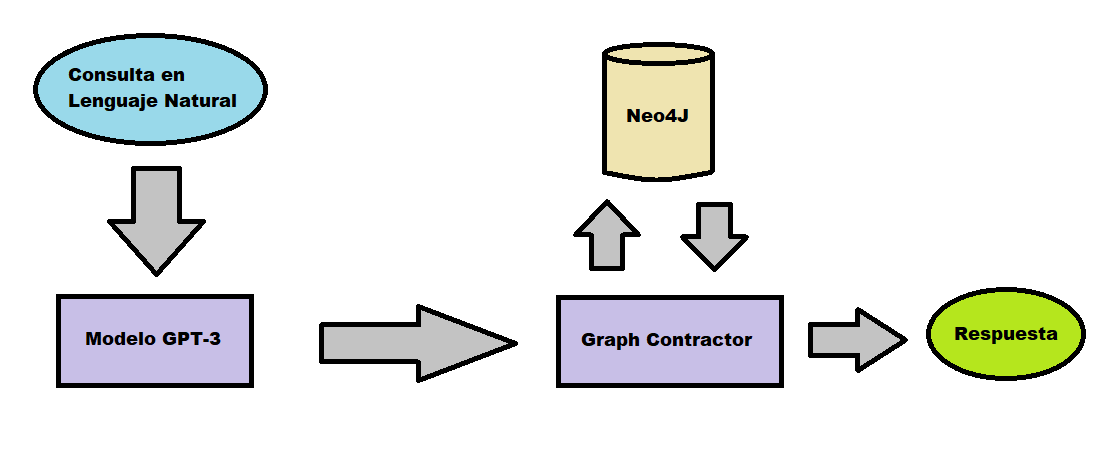
\includegraphics[width=0.5\textwidth]{img/architecture.png}
\caption{Arquitectura del experimento.}\label{img:arch}
\end{figure}

\subsection{Resultados Experimentales}
Para evaluar la calidad de la propuesta de solución se generaron $108$ casos de prueba en forma de pares de consultas en lenguaje natural con su código de \textit{Cypher} correspondiente. Todas las consultas de \textit{Cypher} generadas por el modelo fueron correctamente compiladas, y  de estas, $49$ ($45.37\%$) dieron exactamente la misma respuesta que las consultas de prueba al ser ejecutadas sobre la base de datos.

%===================================================================================
% Bibliografía
%-----------------------------------------------------------------------------------
\begin{thebibliography}{99}
%-----------------------------------------------------------------------------------
	
	\bibitem{graph_dbs} Wikipedia. URL: \href{https://en.wikipedia.org/wiki/Graph_database}
	  {https://en.wikipedia.org/wiki/Graph\_database}.
		Consultado en \today.

	\bibitem{neo4j} Neo4J. URL: \href{https://neo4j.com/}
	  {https://neo4j.com/}.
		Consultado en \today.

	\bibitem{cypher} Neo4J. URL: \href{https://neo4j.com/docs/getting-started/current/cypher-intro/}
	  {https://neo4j.com/docs/getting-started/current/cypher-intro/}.
		Consultado en \today.

	\bibitem{zeroshot} Wikipedia. URL: \href{https://en.wikipedia.org/wiki/Zero-shot_learning}
	  {https://en.wikipedia.org/wiki/Zero-shot\_learning}.
		Consultado en \today.

	\bibitem{rba1} Dar, H. S., Lali, M. I., Din, M. U., Malik, K. M., and Bukhari, S. A. C. (2019). \emph{Frameworks for querying databases using natural language: a literature review.}
		arXiv preprint arXiv:1909.01822 (vid. págs. 3, 8-11, 19).

	\bibitem{rnc} Wu, S., Chen, B., Xin, C., Han, X., Sun, L., Zhang, W., Chen, J., Yang, F., and Cai, X. (2021). \emph{From paraphrasing to semantic parsing: Unsupervised semantic parsing via synchronous semantic decoding.}
		arXiv preprint arXiv:2106.06228 (vid. págs. 2, 7, 8).

	\bibitem{rnr} Cai, R., Yuan, J., Xu, B., and Hao, Z. (2021). \emph{SADGA: Structure-Aware Dual Graph
	Aggregation Network for Text-to-SQL.}
		Advances in Neural Information Processing Systems, 34, 7664-7676 (vid. págs. 2, 7-9).

	\bibitem{comp} Nie, L., Cao, S., Shi, J., Tian, Q., Hou, L., Li, J., and Zhai, J. (2022). \emph{Unifying Semantic Parsing of Graph Query Language with Intermediate Representation.}
		arXiv preprint arXiv:2205.12078 (vid. págs. 7-9).

	\bibitem{transformers} Bazaga, A., Gunwant, N., and Micklem, G. (2021). \emph{Translating synthetic natural lan-
	guage to database queries with a polyglot deep learning framework.}
		Scientific Reports, 11 (1), 1-11 (vid. págs. 6-8).

	\bibitem{gpt3} Wikipedia. URL: \href{https://es.wikipedia.org/wiki/GPT-3}
	  {https://es.wikipedia.org/wiki/GPT-3}.
		Consultado en \today.

	\bibitem{dbschema} IBM. URL: \href{https://www.ibm.com/topics/database-schema}
	  {https://www.ibm.com/topics/database-schema}.
		Consultado en \today.

		\bibitem{moviesdb} Neo4J. URL: \href{https://neo4j.com/docs/getting-started/current/appendix/example-data/}
	  {https://neo4j.com/docs/getting-started/current/appendix/example-data/}.
		Consultado en \today.

%-----------------------------------------------------------------------------------
\end{thebibliography}

%-----------------------------------------------------------------------------------

\end{document}

%===================================================================================
